\chapter{Matlab code}
\section{Part 1}
\subsection{Spatial Cross Correlation in 1d}
\lstinputlisting{code/part1/spatial_correlation_1d.m} \label{code:1.1_1}

\subsection{Normalized Spatial Cross Correlation in 1d}
\lstinputlisting{code/part1/normalised_spatial_correlation_1d.m} \label{code:1.1_2}

\subsection{Signal Offset}
\lstinputlisting{code/part1/signal_offset_checker.m} \label{code:1.2}

\subsection{Normalized Spatial Cross Correlation in 2d}
\lstinputlisting{code/part1/normalised_spatial_correlation_2d.m} \label{code:1.3}

\subsection{Image Alignment}
\lstinputlisting{code/part1/find_the_rocket_man.m} \label{code:1.4}

\subsection{Spectral Cross Correlation}
\lstinputlisting{code/part1/spectral_correlation_function.m} \label{code:1.5}

\subsection{Pattern Finder}
\lstinputlisting{code/part1/pattern_finder.m} \label{code:1.6}

\section{Part 2}
\subsection{Dot Detection Algorithm}
\lstinputlisting{code/part2/dot_detect.m} \label{code:2.1}

\subsection{Create Calibration Model}
\lstinputlisting{code/part2/calibration_model.m} \label{code:2.2}

\subsection{Image Comparison}
\lstinputlisting{code/part2/image_compare.m} \label{code:2.3}

\subsection{Cross Correlation Optimization}
\lstinputlisting{code/part2/image_compare_optimized.m} \label{code:2.4}

\subsection{Multi-pass Cross Correlation}
\lstinputlisting{code/part2/image_compare_multipass.m} \label{code:2.5}

\subsection{Test Scan}
\lstinputlisting{code/part2/test_scan1.m} \label{code:2.6}

\subsection{Optimized Test Scan}
\lstinputlisting{code/part2/test_scan.m} \label{code:2.7}

\subsection{Sub-pixel Dot Detection}
\lstinputlisting{code/part2/subpixel_dot_detect.m} \label{code:2.8}

\section{Part 3}
\subsection{Convolutional Neural Network}
\lstinputlisting{code/part3/number_cnn.m} \label{code:3.1}

\chapter{Test Scan Result}\label{fig:all_test_scan}
\begin{figure}[h!]
	\centering
	\begin{subfigure}[t]{0.3\linewidth}
		\centering
		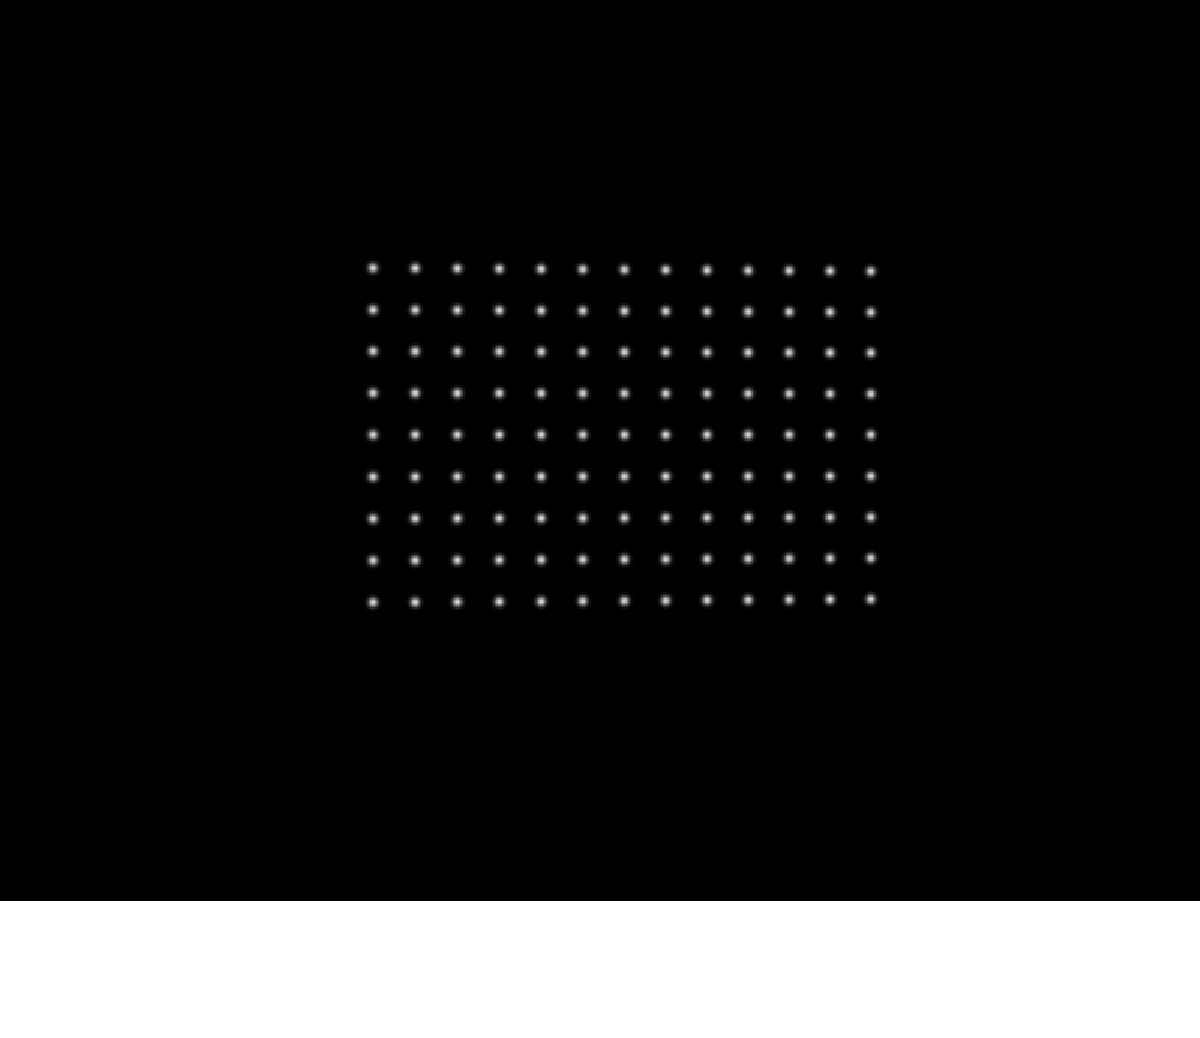
\includegraphics[width=0.8\linewidth]{figures/part2/test_left_1}
	\end{subfigure}
	\begin{subfigure}[t]{0.3\linewidth}
		\centering
		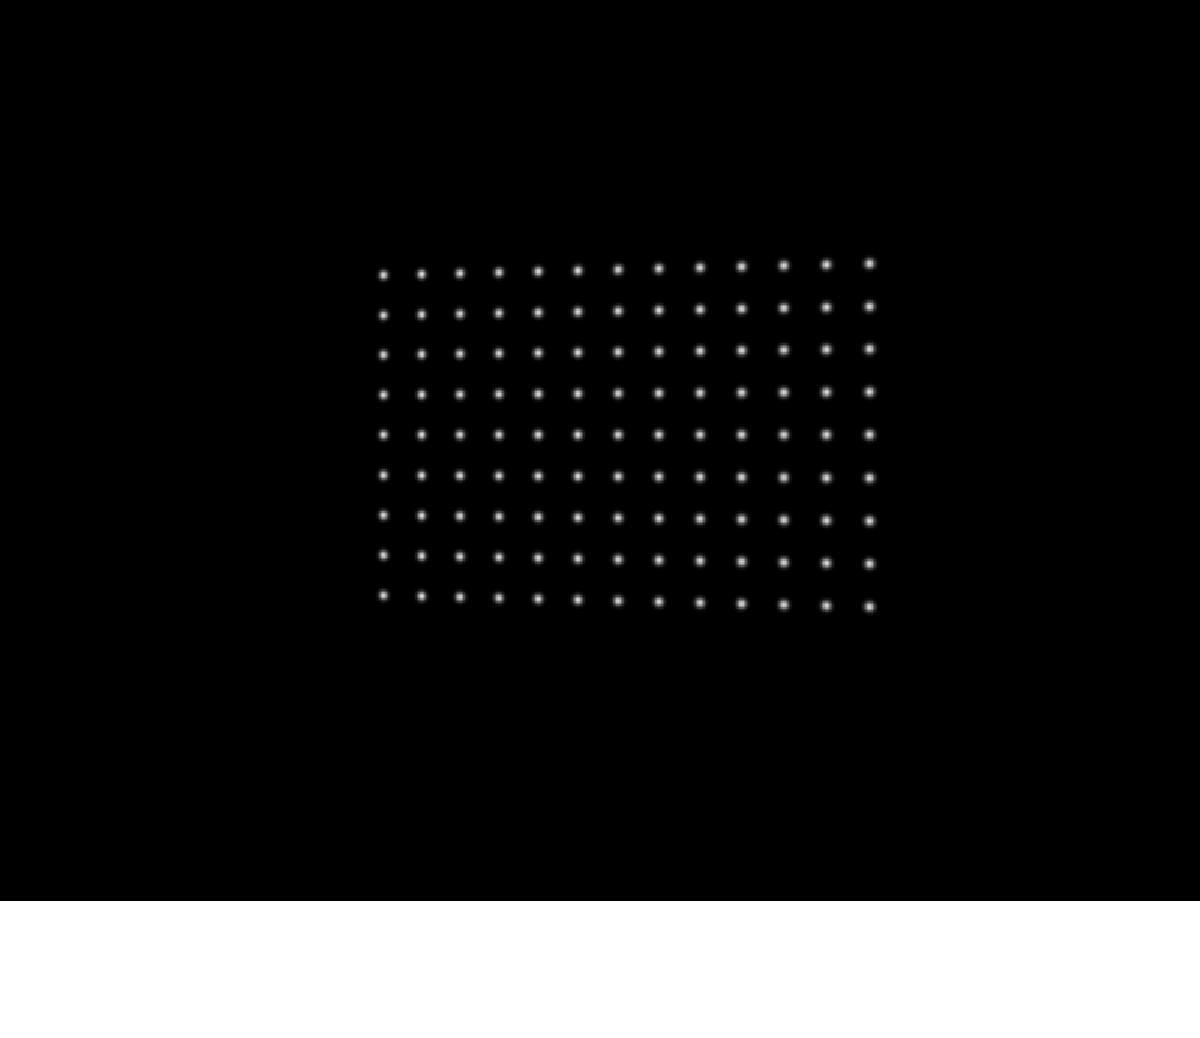
\includegraphics[width=0.8\linewidth]{figures/part2/test_right_1}
	\end{subfigure}
	\begin{subfigure}[t]{0.35\linewidth}
		\centering
		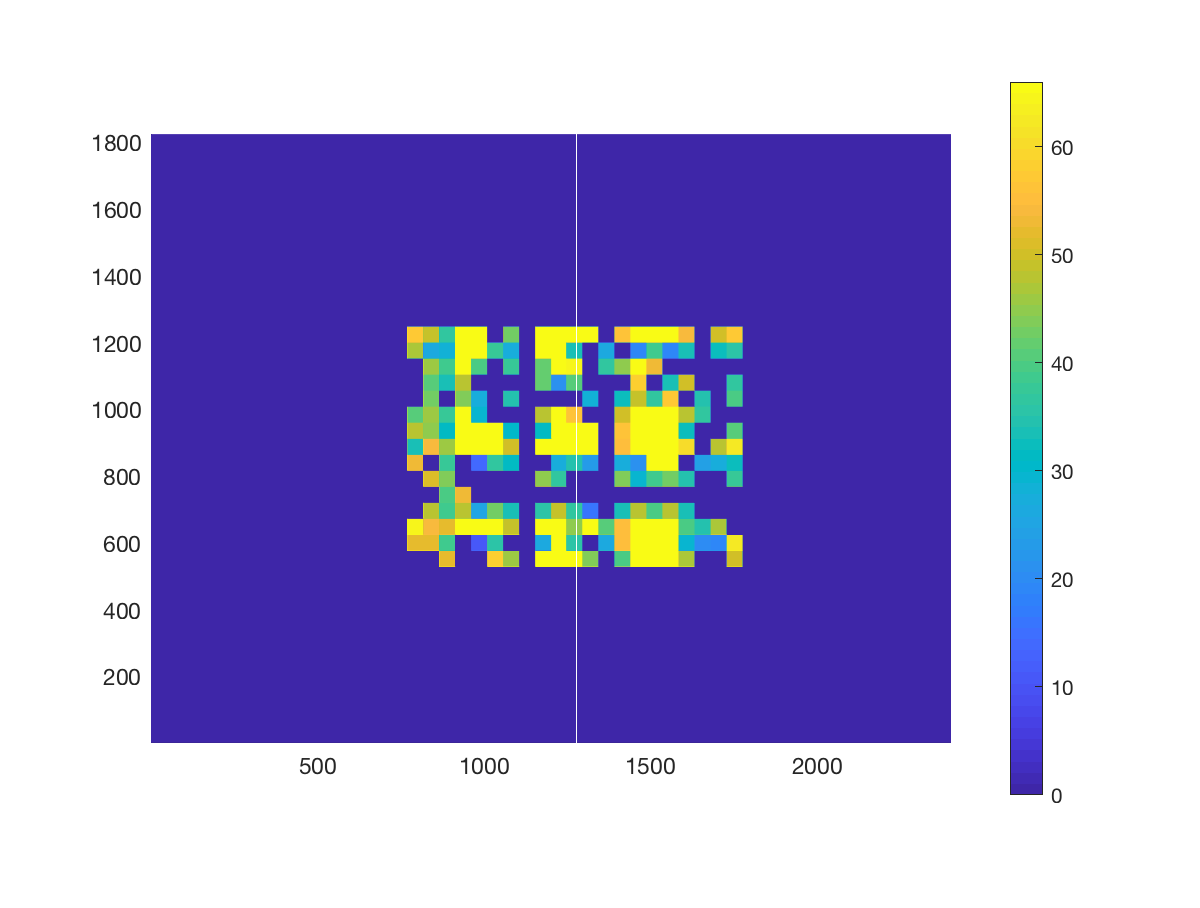
\includegraphics[width=1\linewidth]{figures/part2/test1_cmp}
	\end{subfigure}
	\begin{subfigure}[t]{0.45\linewidth}
		\centering
		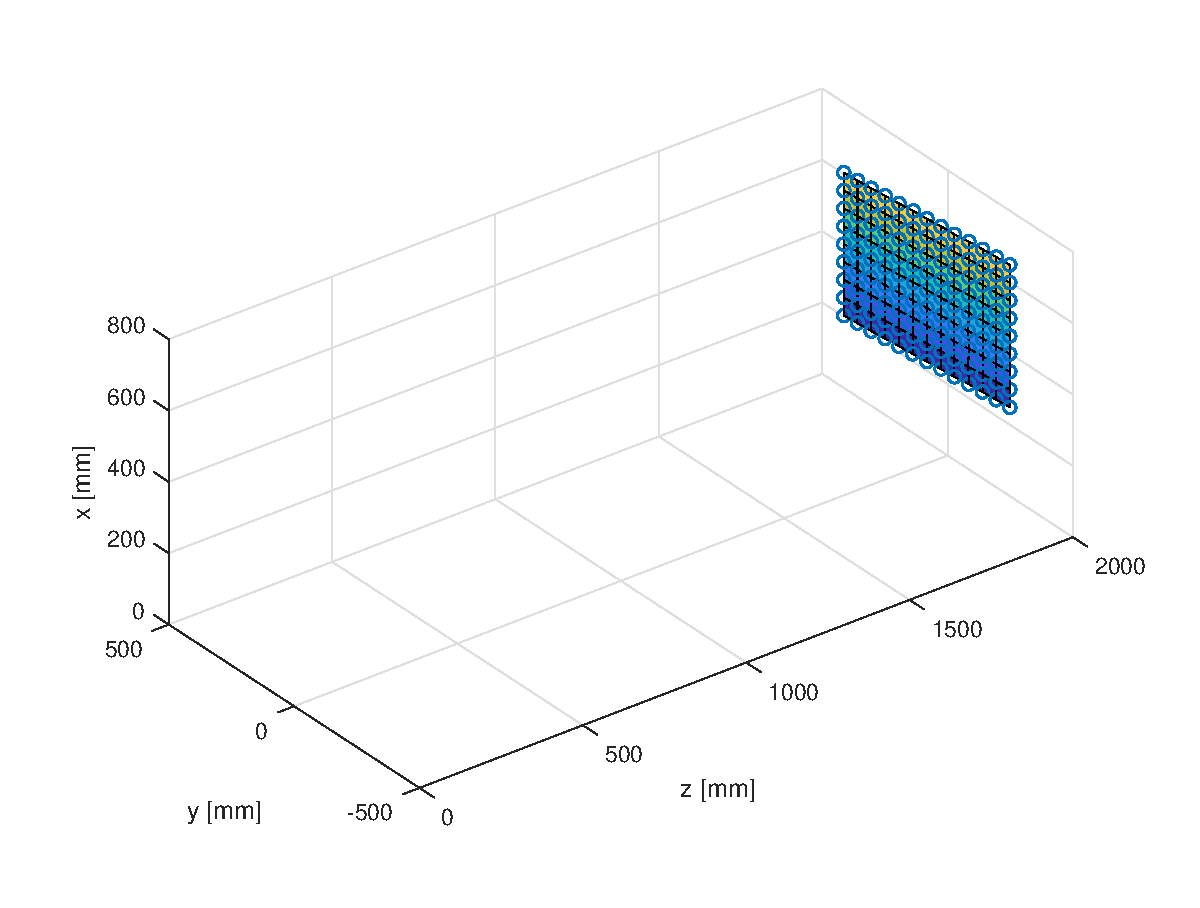
\includegraphics[width=1\linewidth]{figures/part2/test1_scan}
	\end{subfigure}
	\begin{subfigure}[t]{0.45\linewidth}
		\centering
		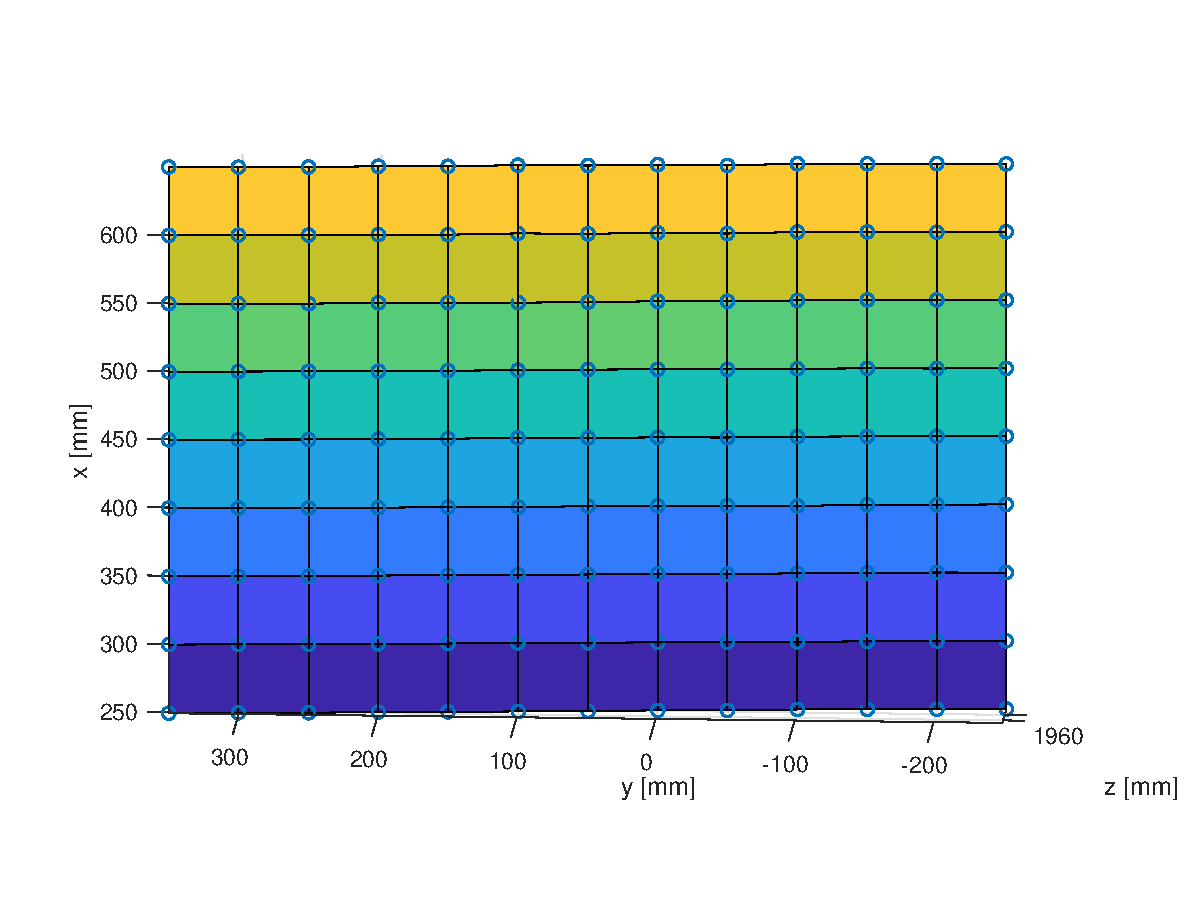
\includegraphics[width=1\linewidth]{figures/part2/test1_scan1}
	\end{subfigure}
	\caption{Test scan on image pair 1}
\end{figure}
\begin{figure}[h!]
	\begin{subfigure}[t]{0.3\linewidth}
		\centering
		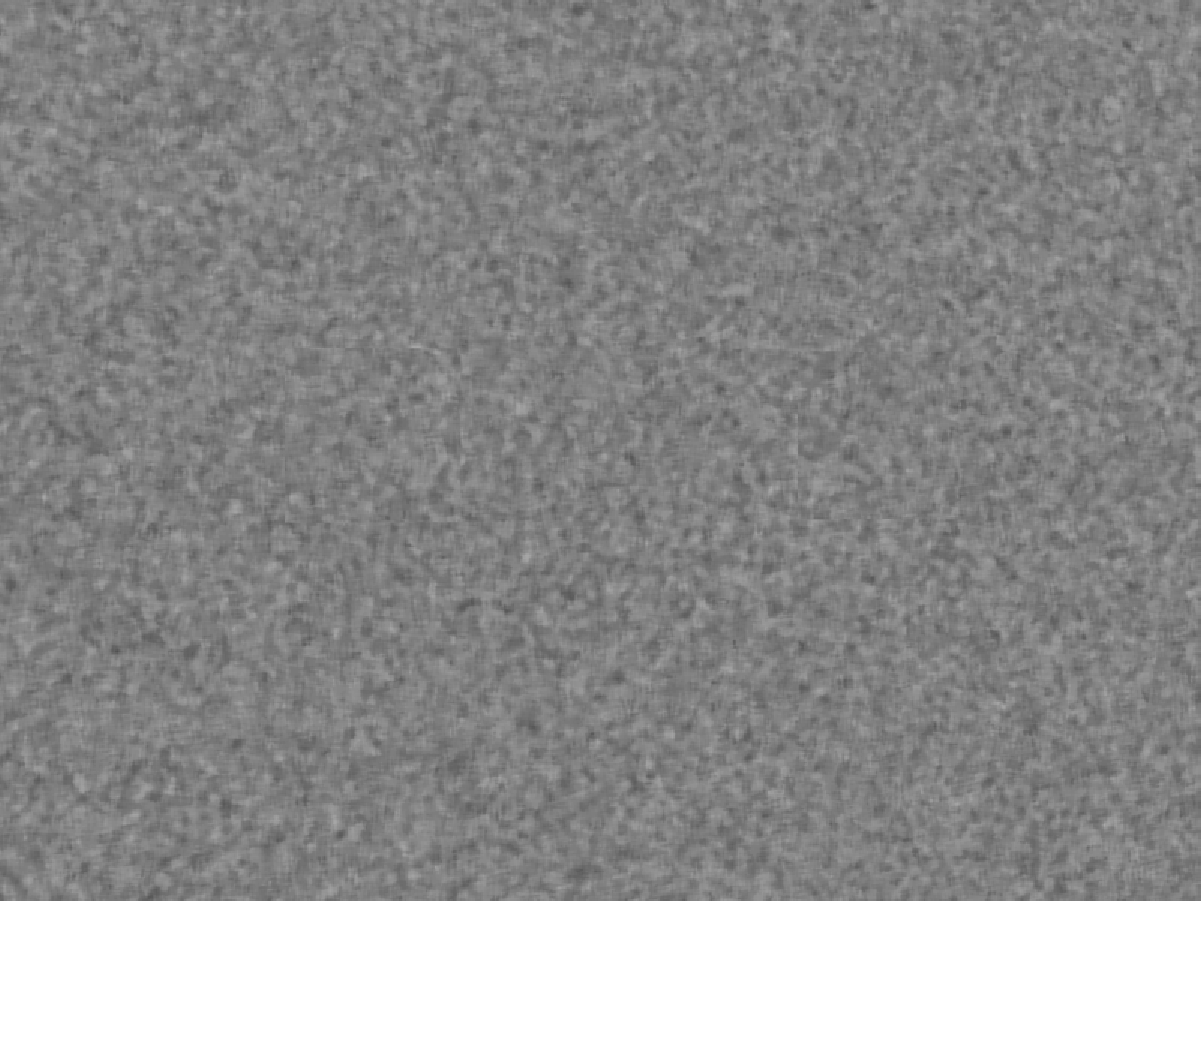
\includegraphics[width=0.8\linewidth]{figures/part2/test_left_2}
	\end{subfigure}
	\begin{subfigure}[t]{0.3\linewidth}
		\centering
		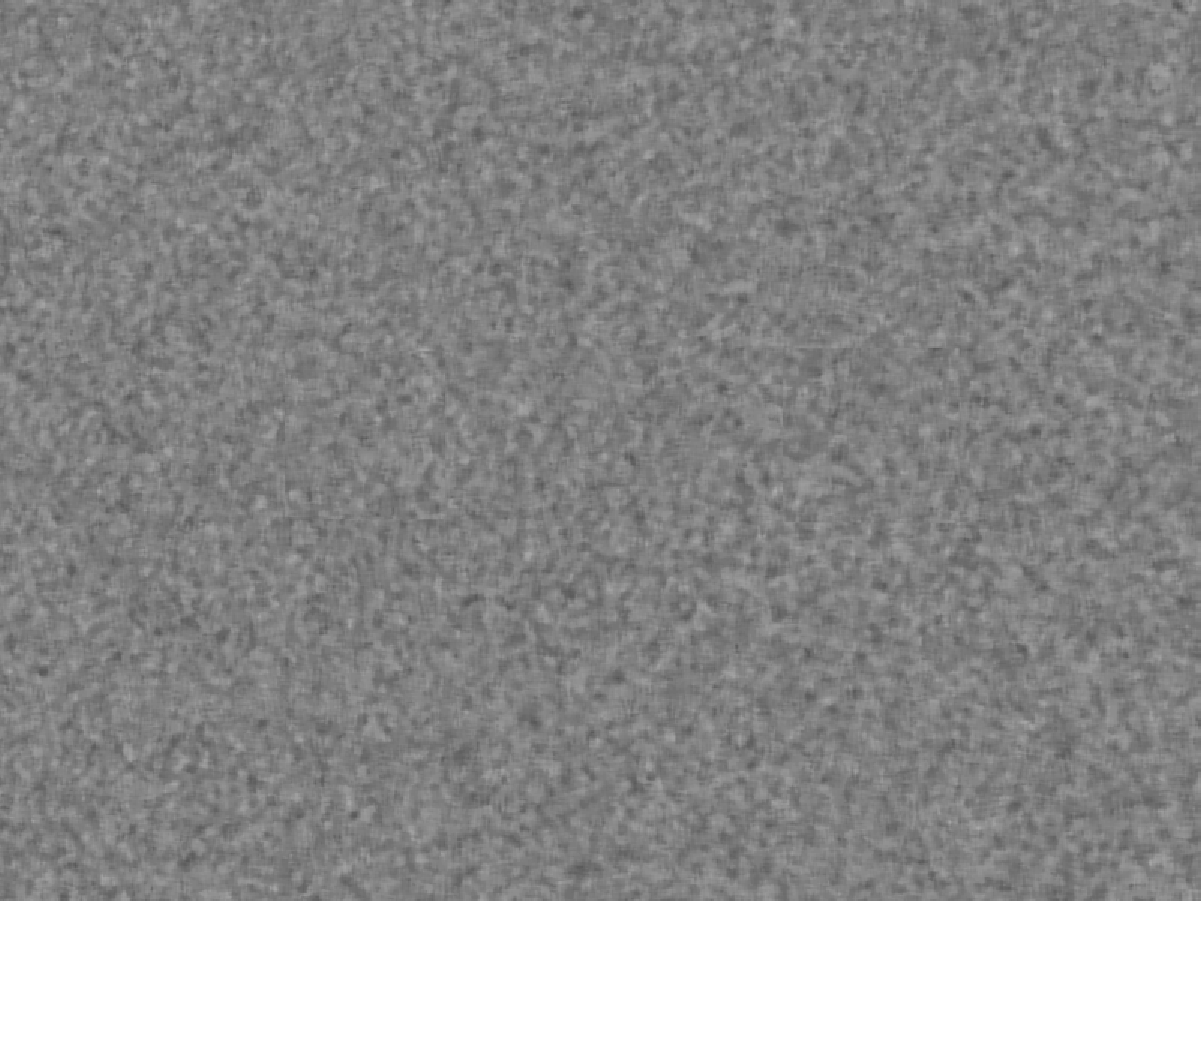
\includegraphics[width=0.8\linewidth]{figures/part2/test_right_2}
	\end{subfigure}
	\begin{subfigure}[t]{0.35\linewidth}
		\centering
		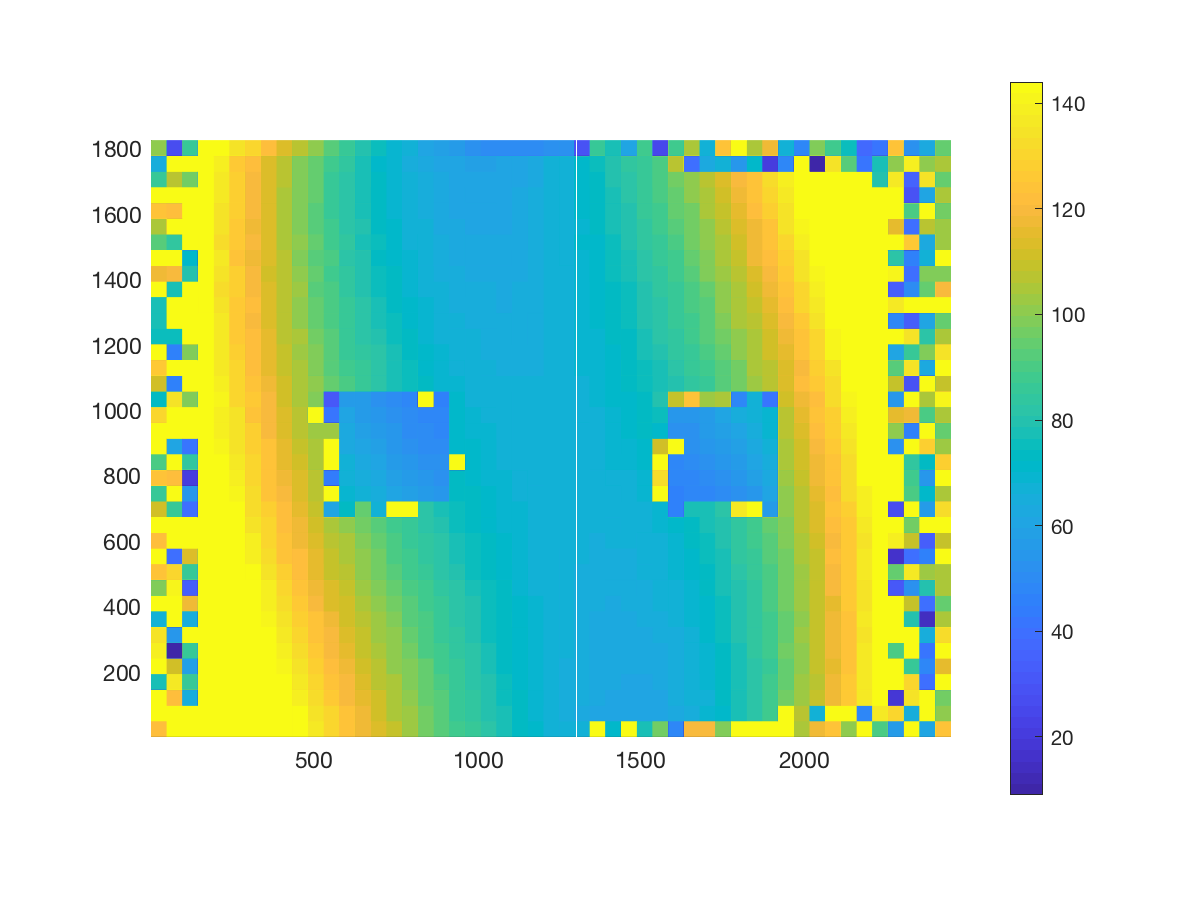
\includegraphics[width=1\linewidth]{figures/part2/test2_cmp}
	\end{subfigure}
	\begin{subfigure}[t]{0.45\linewidth}
		\centering
		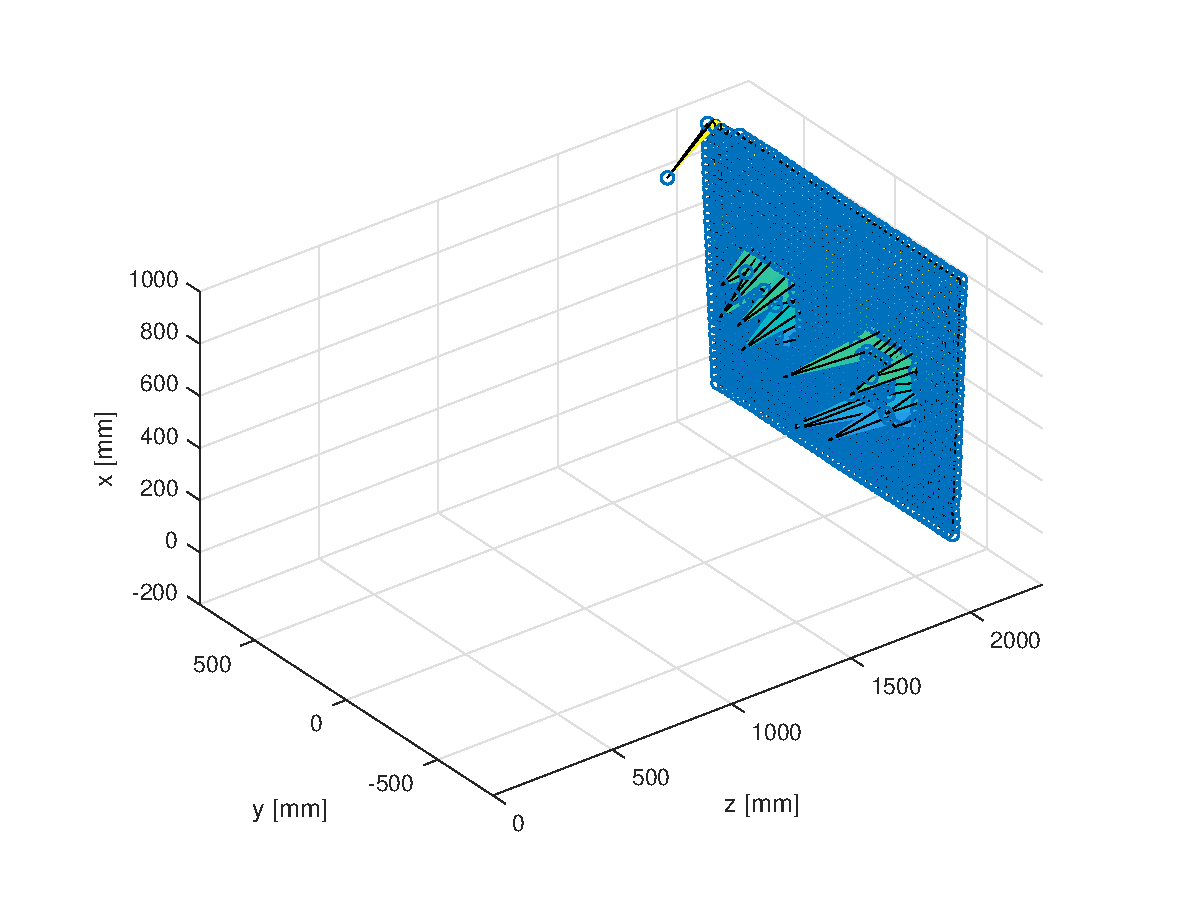
\includegraphics[width=1\linewidth]{figures/part2/test2_scan}
	\end{subfigure}
	\begin{subfigure}[t]{0.45\linewidth}
		\centering
		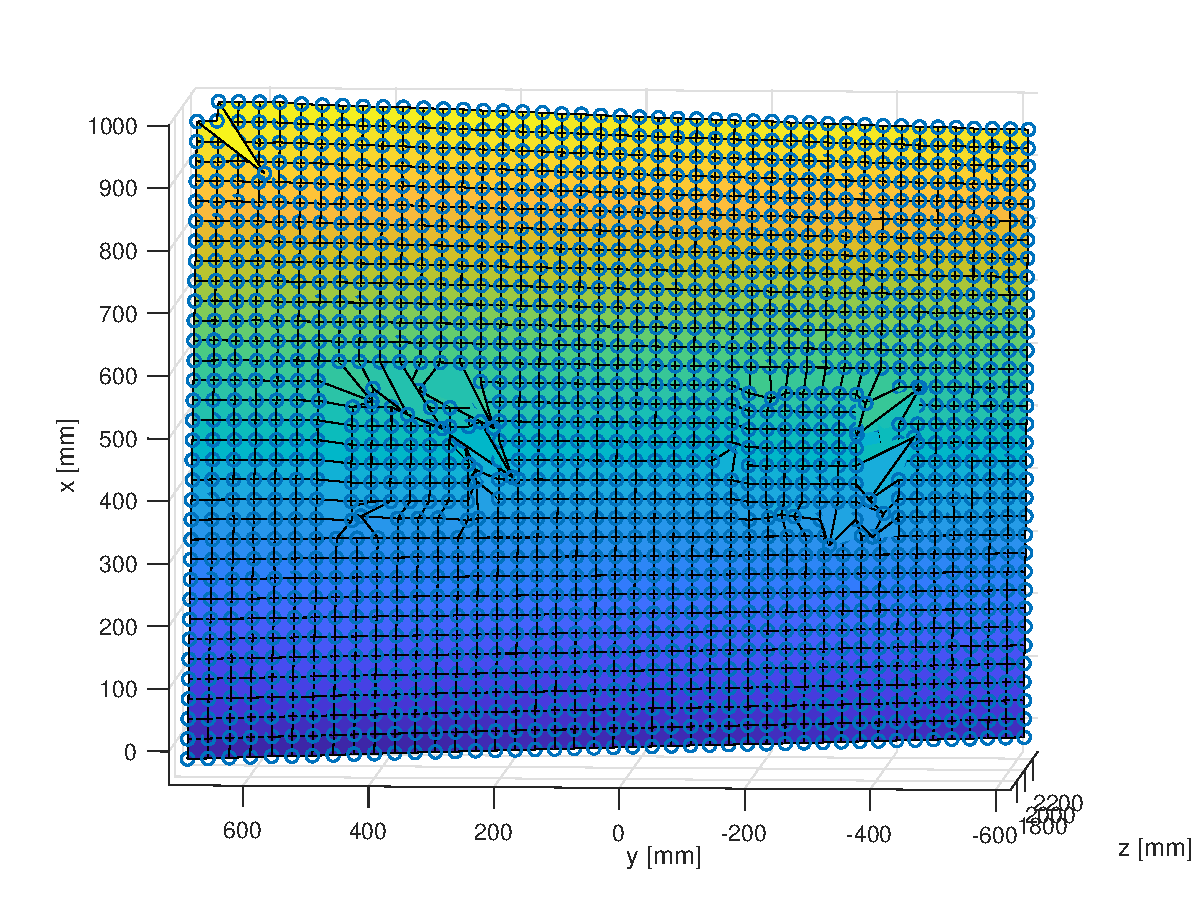
\includegraphics[width=1\linewidth]{figures/part2/test2_scan1}
	\end{subfigure}
	\caption{Test scan on image pair 2}
\end{figure}
\begin{figure}[h!]
	\begin{subfigure}[t]{0.3\linewidth}
		\centering
		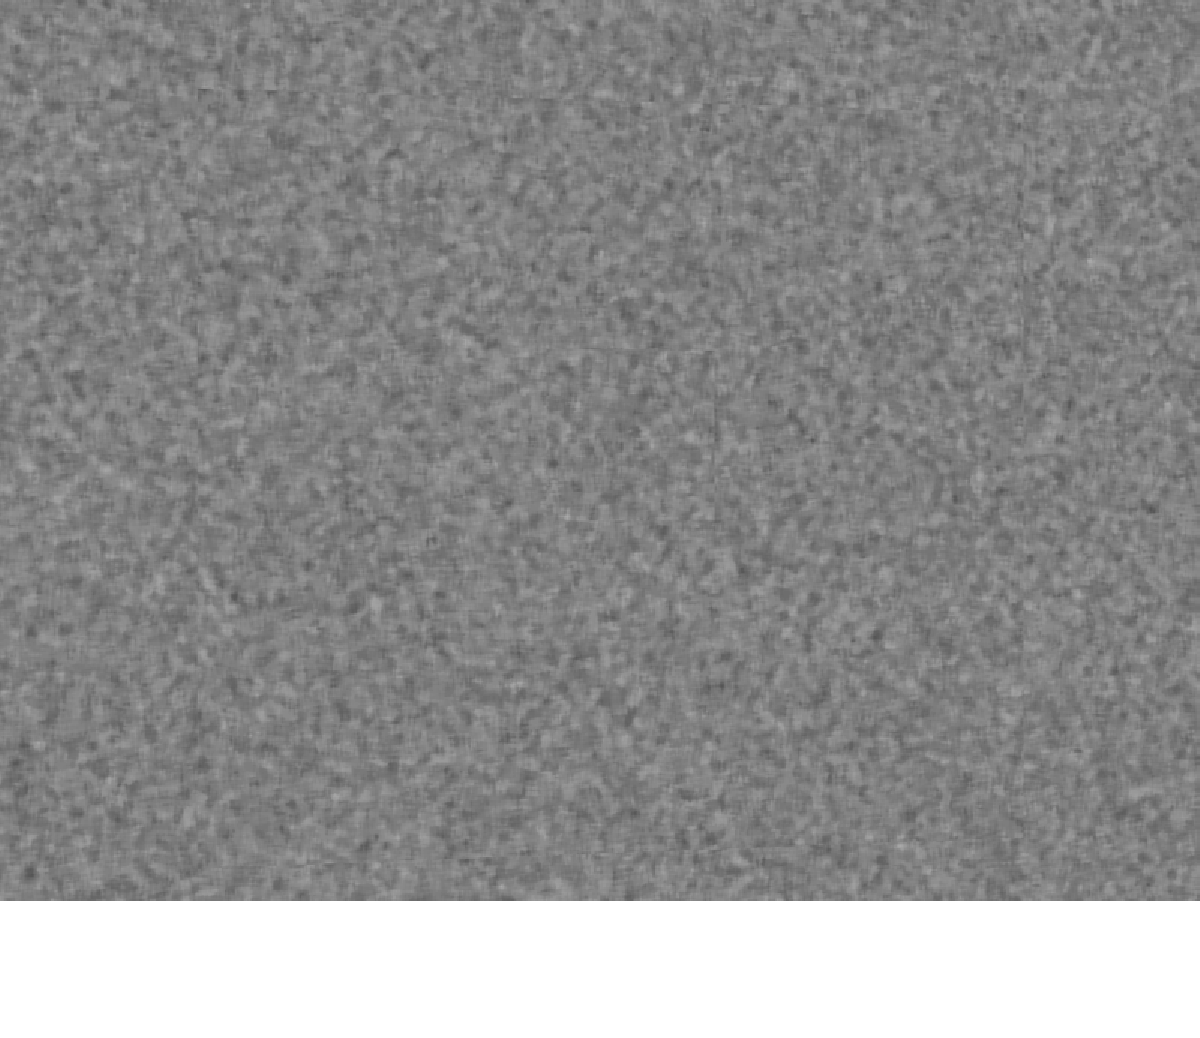
\includegraphics[width=0.8\linewidth]{figures/part2/test_left_3}
	\end{subfigure}
	\begin{subfigure}[t]{0.3\linewidth}
		\centering
		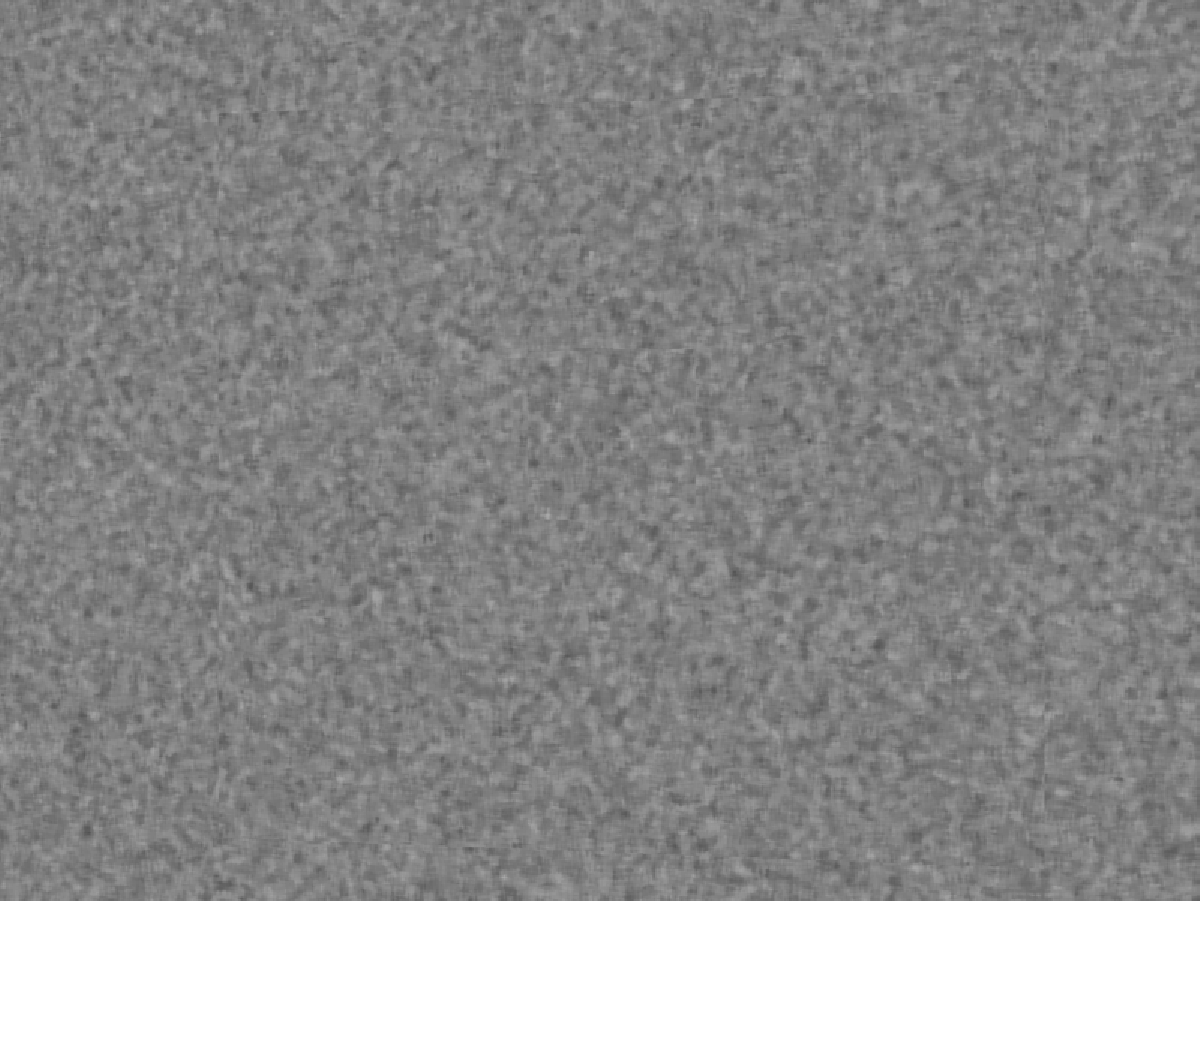
\includegraphics[width=0.8\linewidth]{figures/part2/test_right_3}
	\end{subfigure}
	\begin{subfigure}[t]{0.35\linewidth}
		\centering
		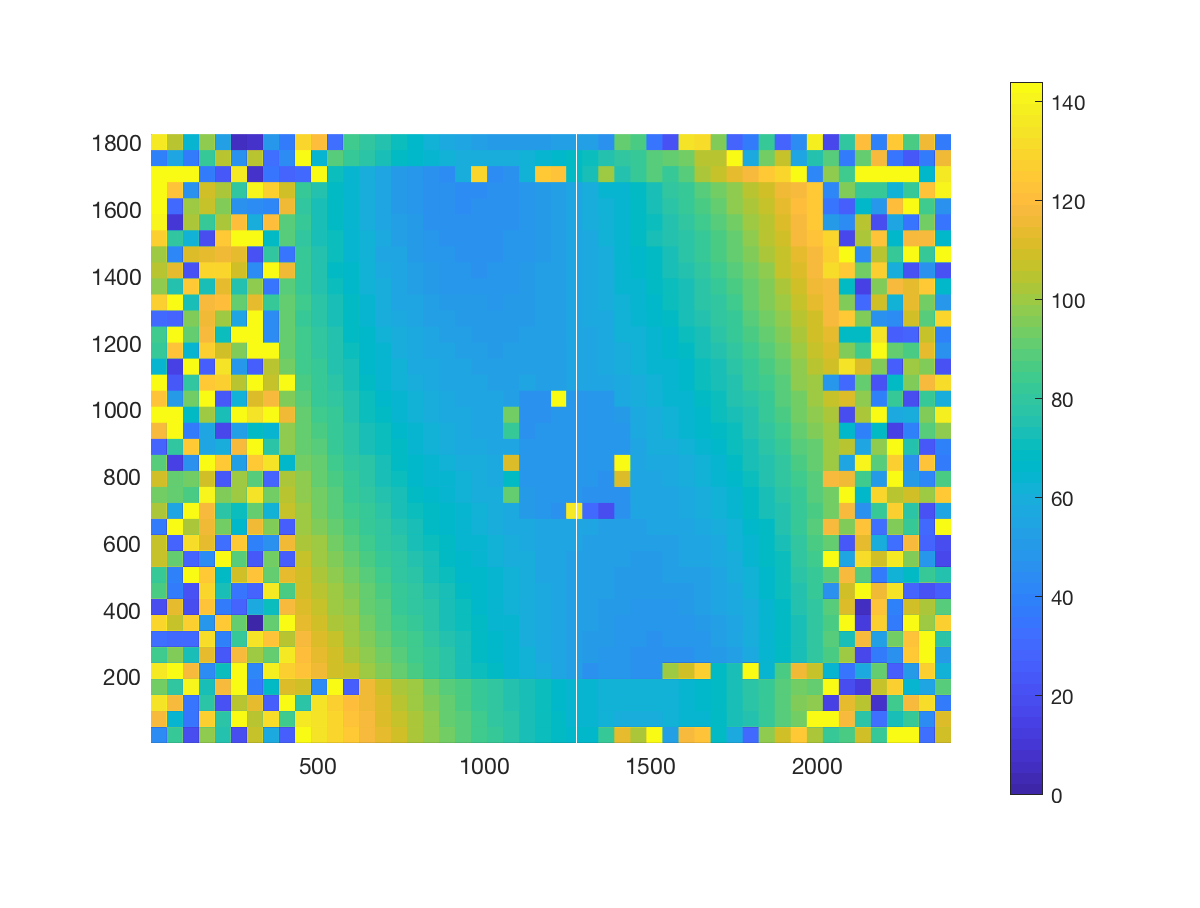
\includegraphics[width=1\linewidth]{figures/part2/test3_cmp}
	\end{subfigure}
	\begin{subfigure}[t]{0.45\linewidth}
		\centering
		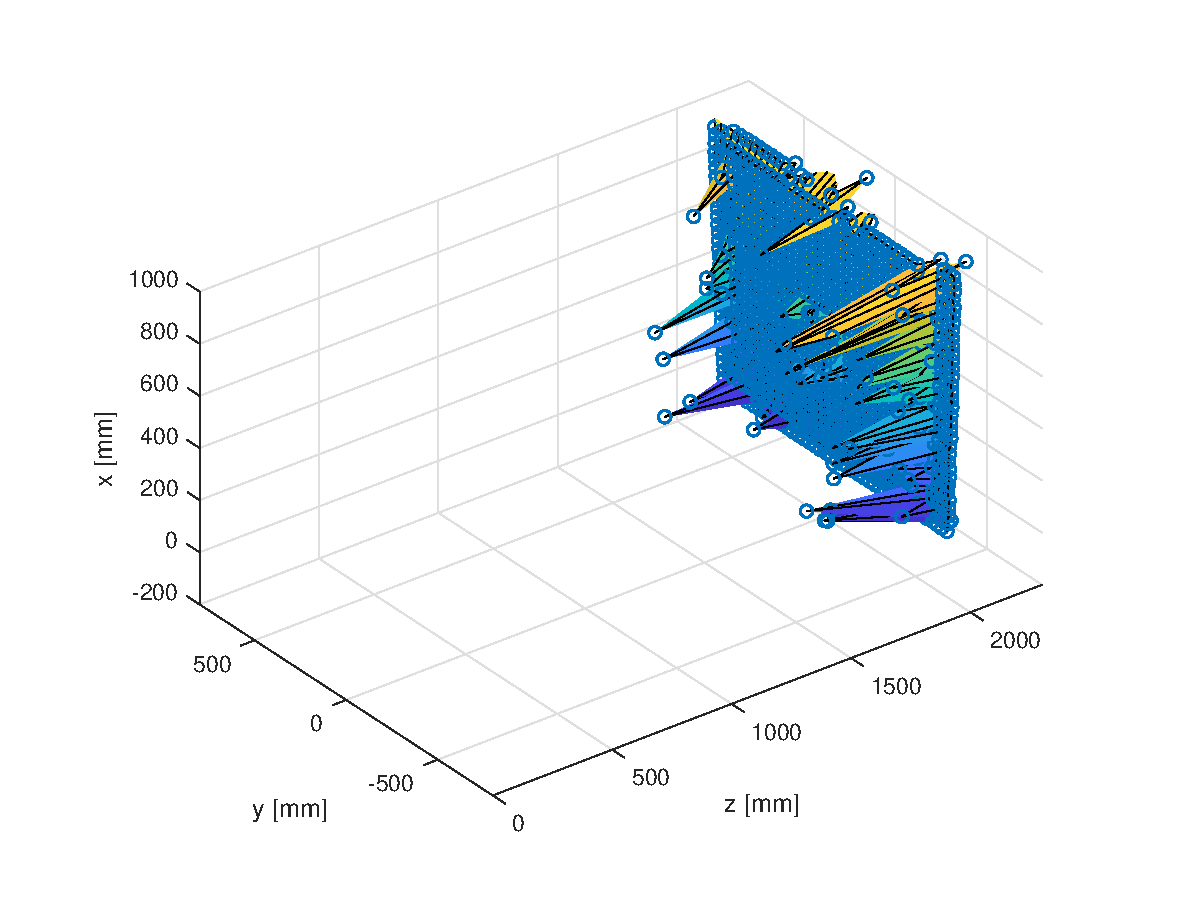
\includegraphics[width=1\linewidth]{figures/part2/test3_scan}
	\end{subfigure}
	\begin{subfigure}[t]{0.45\linewidth}
		\centering
		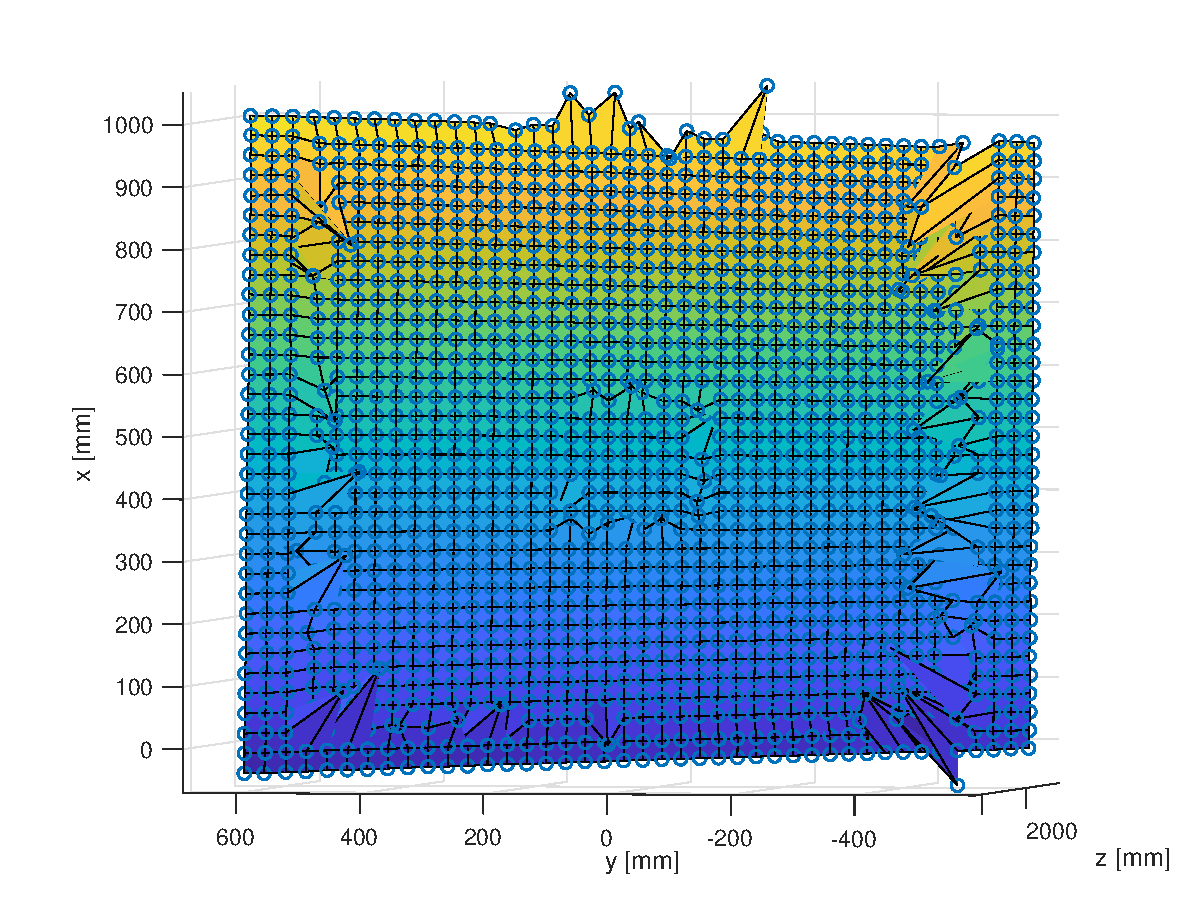
\includegraphics[width=1\linewidth]{figures/part2/test3_scan1}
	\end{subfigure}
	\caption{Test scan on image pair 3}
\end{figure}